\documentclass[
% -- opções da classe memoir --
article,			% indica que é um artigo acadêmico
12pt,				% tamanho da fonte
oneside,			% para impressão apenas no recto. Oposto a twoside
a4paper,			% tamanho do papel. 
english,			% idioma adicional para hifenização
brazil,				% o último idioma é o principal do documento
sumario=tradicional
]{abntex2}

% ---
% PACOTES
% ---
\usepackage{lmodern} % Usa a fonte Latin Modern
\usepackage[T1]{fontenc}% Selecao de codigos de fonte.
\usepackage[utf8]{inputenc}% Codificacao do documento (conversão automática dos acentos)
\usepackage{indentfirst}% Indenta o primeiro parágrafo de cada seção.
\usepackage{nomencl} % Lista de simbolos
\usepackage{color}% Controle das cores
\usepackage{graphicx}% Inclusão de gráficos
\usepackage{microtype}% para melhorias de justificação
\usepackage{gensymb}
\usepackage{caption}
\usepackage{booktabs}
\usepackage{footnote}
\usepackage{listings}
\usepackage{longtable}

\definecolor{dkgreen}{rgb}{0,0.6,0}
\definecolor{gray}{rgb}{0.5,0.5,0.5}
\definecolor{mauve}{rgb}{0.58,0,0.82}

\lstset{frame=tb,
  language=C++,
  aboveskip=3mm,
  belowskip=3mm,
  showstringspaces=false,
  columns=flexible,
  basicstyle={\small\ttfamily},
  numbers=left,
  numberstyle=\tiny\color{gray},
  keywordstyle=\color{blue},
  commentstyle=\color{dkgreen},
  stringstyle=\color{mauve},
  breaklines=true,
  breakatwhitespace=true,
  tabsize=4
}

% ---
% Pacotes adicionais, usados apenas no âmbito do Modelo Canônico do abnteX2
% ---
% ---
% Pacotes de citações
% ---
\usepackage[brazilian,hyperpageref]{backref}	 % Paginas com as citações na bibl
%\usepackage[alf,abnt-emphasize=bf]{abntex2cite}	% Citações padrão ABNT
\usepackage[num,overcite,abnt-emphasize=bf]{abntex2cite}	% Citações padrão ABNT
%\citebrackets()
\citebrackets[]
% ---

% ---
% Configurações do pacote backref
% Usado sem a opção hyperpageref de backref
\renewcommand{\backrefpagesname}{Citado na(s) página(s):~}
% Texto padrão antes do número das páginas
\renewcommand{\backref}{}
% Define os textos da citação
\renewcommand*{\backrefalt}[4]{
  \ifcase #1 %
    Nenhuma citação no texto.%
    \or
    Citado na página #2.%
  \else
    Citado nas páginas #2.%
\fi}%
% ---

\graphicspath{{./images/}}

% --- Informações de dados para CAPA e FOLHA DE ROSTO ---
\titulo{IoT: rede LoRa para envio de imagens}
\tituloestrangeiro{IoT: LoRa network for sending images}


\autor{Victor E. Almeida \and Marco A. Guerra}
%\autor{
  %UNIOESTE\thanks{``Universidade Estadual do Oeste do Paraná, Foz do Iguaçu, Brasil.'' \url{http://www.unioeste.br/}} 
  %\\[0.5cm]\\
  %Victor Emanuel Almeida\thanks{``Estudante de Ciência da Computação na Universidade Estadual do Oeste do Paraná (UNIOESTE), campus de Foz do Iguaçu-PR, Brasil.''\url{http://www.unioeste.br/}}
%}



\local{Foz do Iguaçu}
\data{\today}

\instituicao{%
\par
Universidade do Oeste do Paraná 
\par
UNIOESTE
}
\instituicao{Curso de Ciência da Computação, da Universidade Estadual do Oeste do Paraná (UNIOESTE), Campus Foz do Iguaçu-PR, Brasil}

\preambulo{Escrever Preâmbulo}

\tipotrabalho{Trabalho Acadêmico}
% ---

% ---
% Configurações de aparência do PDF final

% alterando o aspecto da cor azul
\definecolor{blue}{RGB}{41,5,195}

% informações do PDF
\makeatletter
\hypersetup{
  %pagebackref=true,
  pdftitle={\@title}, 
  pdfauthor={\@author},
  pdfsubject={software livre},
  pdfcreator={\@author},
  pdfkeywords={software livre},
  colorlinks=true,% false: boxed links; true: colored links
  linkcolor=black,% color of internal links
  citecolor=blue,% color of links to bibliography
  filecolor=magenta,% color of file links
  urlcolor=blue,
  bookmarksdepth=4
}
\makeatother
% --- 

% ---
% compila o indice
% ---
\makeindex
% ---

% ---
% Altera as margens padrões
% ---
\setlrmarginsandblock{3cm}{2cm}{*}
\setulmarginsandblock{3cm}{2cm}{*}
\checkandfixthelayout
% ---

% --- 
% Espaçamentos entre linhas e parágrafos 
% --- 

% O tamanho do parágrafo é dado por:
\setlength{\parindent}{1.25cm}
%\setlength{\parindent}{1.5\lineheight}

% Controle do espaçamento entre um parágrafo e outro:
%\setlength{\parskip}{0.2cm}  % tente também \onelineskip
\setlength{\parskip}{\onelineskip}

% Espaçamento simples
\SingleSpacing

% ----
% Início do documento
% ----
\begin{document}
%\pagenumbering{roman}
% Seleciona o idioma do documento (conforme pacotes do babel)
%\selectlanguage{english}
\selectlanguage{brazil}

% Retira espaço extra obsoleto entre as frases.
\frenchspacing 

% ----------------------------------------------------------
% ELEMENTOS PRÉ-TEXTUAIS
% ----------------------------------------------------------

%---
%
% Se desejar escrever o artigo em duas colunas, descomente a linha abaixo
% e a linha com o texto ``FIM DE ARTIGO EM DUAS COLUNAS''.
%\twocolumn[    		% INICIO DE ARTIGO EM DUAS COLUNAS
%
%---

% página de titulo principal (obrigatório)
%\imprimircapa
%\begin{center}
\maketitle
%{\centered\maketitle\imprimirlocal\imprimirinstituicao}
%\imprimirtitulo
%\vspace{.5cm}

%\imprimirinstituicao
%\end{center}

% titulo em outro idioma (opcional)

% resumo em português
\begin{resumoumacoluna}
    % De 100 a 250 palavras
    % frases curtas
    % tem que falar de:
        % objetivo
        % matérias e métodos
        % resultados
        % concluir
  \textbf{Palavras-chave}: LoRa, Rede LPWAN, envio de imagens.
  \vspace{\onelineskip}
  \noindent
\end{resumoumacoluna}

% resumo em inglês
\renewcommand{\resumoname}{Abstract}
\begin{resumoumacoluna}
  \begin{otherlanguage*}{english}
    Escrever resumo
    \vspace{\onelineskip}
    \noindent

    \textbf{Keywords}: LoRa, LPWAN Network, sending images.
  \end{otherlanguage*}  
\end{resumoumacoluna}

\cleardoublepage

%] % FIM DE ARTIGO EM DUAS COLUNAS
% ---

% ----------------------------------------------------------
% ELEMENTOS TEXTUAIS
% ----------------------------------------------------------

\textual

% ----------------------------------------------------------
% Introdução
% ----------------------------------------------------------

\section{Introdução}
O barateamento dos dispositivos de Internet of Thing tem aberto novas possíbilidaes, ainda com a adquisição de novas capacidades com um menor consumo de energia e maior eficiência tem se torndo possível a implementação de sistemas embarcados cada vez mais específicos a um baixo custo.

Nesse sentido, uma das carateristicas desejáveis nos dispositivos e o envio de dados a longa distãncia, para

O seguinte trabalho apresenta as princiapis escolhas e os resultados obtidos na implementação do uma rede baseada em LoRa para o envio de imagens entre dispositivos 

\section{Definições}
Antes de abordar as principais tecnologias, bem como os principais algoritmos utilizados durante o projeto, faz-se necessário elucidar alguns pontos.

\subsection{LoRa}
Os dispositivos LoRa são uma implementação da camada física do modelo OSI para o envio e recevimento de dados. Criado e mantido de forma proprietária pela empresa Semtech o mesmo utiliza comunicação atraves de ondas na frequência de radio, para codificar o envio de dados focando em abarcar longas distãncia a um baixo custo energetico. Nesse sentido, uma rede LoRa é formada por diversas antenas\cite{siteLorawan}, que se comunicam utilizando a tecnologia de \textit{Chirp Spread Spectrum}\cite{davcev2018iot} uma tecnologia de comunicação militar adaptada para uso comercial de baixo custo\cite{siteLorawan} tais antenas possuem alcance de até 15 km em áreas rurais\cite{adelantado2017understanding}, bem como uma taxa média de duração de bateria de 10 anos\cite{adelantado2017understanding}.

\subsection{IoT}
O termo \textit{Internet of Things (IOT)}, em português internet das coisas foi elaborado pelo britânico, Kevin Ashton, em 1999\cite{tzounis2017internet} e se refere de forma geral a uma rede que conecta diversas ``coisas'' a internet, através de software, com o objetivo de trocar informações\cite{defIot}, tais ``coisas'' podem ser sensores, microcontroladores ou até mesmo objetos que nunca imaginamos tais como geladeiras, televisores, entre outros.

A estrutura do \textit{internet of things} é baseada em três camadas principais\cite{tzounis2017internet}:
\begin{itemize}
	\item \textbf{Camada de percepção}: É uma camada que envolve sensores, hardware e obtém-se dados relevantes a respeito dos fenômenos meteorológicos, biológicos ou físicos tais como  temperatura e umidade do solo\cite{kizito2008frequency}, do ar\cite{mesas2015open}, índice de área foliar\cite{bauer2016potential}, quantidade de gás SO$_{2}$\cite{karimi2018web}, PH do solo\cite{karimi2018web} entre muitos outros.
	\item \textbf{Camada de comunicação}: Responsável por enviar os dados coletados pela camada de percepção supracitada para outras camadas, quer sejam aplicações que vão analisar tais dados ou para grandes bancos de dados ou até mesmo para serviços na nuvem.
	\item \textbf{Camada de aplicação}: camada a qual trás sentido aos dados coletados pelos sensores, pois é nesse momento que ocorre o processamento dos dados e a apresentação dos mesmos. Nos trabalhos lidos durante a produção desta revisão bibliográfica, essa camada será responsável principalmente por mostrar ao agricultor informações relevantes de forma simples e compreensível, bem como informá-lo qual o melhor momento para plantar\cite{kath2019soil}, ou em quais lugares da plantação tem doenças\cite{trilles2019development}.
\end{itemize}

Ainda pode ser citada uma camada intermediária, sendo ela chamada de \textit{\bfseries Middleware} a qual facilita a interação da camada de aplicação com a de percepção\cite{tzounis2017internet}, fornecendo ferramentas que permitem abstrações em relação a camada de percepção e possibilitando a integração de softwares recentes com o legado\cite{tzounis2017internet}. Um exemplo é na pesquisa de \cite{sawant2017interoperable} essa integração foi feita a partir de um \textit{Web processing Service} que padroniza as entradas e saídas e também por diversos serviços para refinar os dados obtidos dos sensores, fazendo assim o pré-processamento das medições, explicado com muitos detalhes na seção 2.2 de seu trabalho.

\cleardoublepage

\section{Materiais e métodos}\label{Materiais e métodos}

\subsection{Protocolos}\label{Protocolos}

Dados os requisitos do projeto a escolha dos algoritmos proprios para a tarefa a ser desempenhada se torna de extrema relevância. Nesse sentido, são abordados os diferentes algoritmos utilizados na implementação do sistema, dando especial atenção para as caraterísticas que influenciaram na sua escolha.

\subsubsection{Detecção de erros: CRC}\label{CRC}

Visando a detecção de erros um dos algoritmos 

Falar dos algoritmos de Detecção de erro (CRC) e correção de erros (Hamming)

\begin{lstlisting}[title=Algoritmo CRC 16 bits]
static const uint16_t POLY = 0xA001;
static const uint16_t INIT = 0xC181;

uint16_t computeCRC(uint8_t* data_in, uint16_t length) {
    uint16_t i;
    uint8_t bitbang, j;
    uint16_t crc_calc = INIT;

    for(i = 0; i < length; i++) {
        crc_calc ^= (((uint16_t)data_in[i]) & 0x00FF);
        for(j = 0; j < 8; j++) {
            bitbang = crc_calc;
            crc_calc >>= 1;

            if(bitbang & 1) {
                crc_calc ^= POLY;
            }
        }
    }
    return (crc_calc & 0xFFFF);
}
\end{lstlisting}

\subsubsection{Stop and Wait}\label{Stop and Wait}

Do ponto de vista da camada de enlace de dados o algoritmo utilizado foi o \textbf{Stop and Wait}, o qual se carateriza pela sua simplicidade tanto durante a sua implementação como no seu funcionamento. A continuação é descrito o funcionamento dos dispositivos envolvidos no envio e recebimento de imagens.

Do lado do Sender, dispositivo que captura e envia imagens, em um primeiro momento são inicializadas a câmara e a antena LoRa. A continuação é feita a captura de uma imaagen que passa a ser dividida em partes atendendo ao tamanho maximo que pode ter o payload da mensagem que pode ser enviada pela antena LoRa. Assim, uma vez particionada a imagem inicia o seu processo de envio o qual continua se

\begin{lstlisting}[title=Algoritmo Stop and Wait - Sender]
void sender() {
	InitCamera();
	InitLoRa();
	TakePicture(image); // tira uma foto
	SplitImage(image); // separa image em pacotes
	while(image.sendedParts < image.totalParts) {
		SendImagePart(image.part()); // envia quadro contendo parte da imagem
		ReceivePacketCommand	(buffer); // espera ate receber um quadro
		if(buffer.messageType == ACK) {
			image.sendedParts++; // incrementa contador de imagens enviadas
		}
	}
}
\end{lstlisting}

Por outro lado no reciver, em um primeiro momento também são inicializadas as estruturas de controle, bem como é alocado um espaço que serve de buffer para colocar as partes da imagem que está sendo recevida. Apos isso, o dispositivo fica esperando o recevimento de pacotes

\begin{lstlisting}[title=Algoritmo Stop and Wait - Reciver]
void reciver() {
	InitImage(image); // inicializa estrutura de dados das imagens
	InitLoRa();
	while(true) {
		ReceivePacketCommand	(buffer); // espera ate receber um quadro
		SaveImageBytes(buffer); // salvar bytes na estrutura da imagem
		PrepareFrameCommand(); // prepara ACK
		SendPacket(); // envia ACK
		if(image.isComplete()) {
			SaveImage(image); // salvar imagem em arquivo
		}
	}
}
\end{lstlisting}

\cleardoublepage

\subsection{Dispositivos}\label{Dispositivos}

\subsubsection{LoRaMESH EndDivice}\label{LoRaMESH EndDivice}

\begin{figure}[!h]
  \caption{\label{fig:recivier}LoRaMESH EndDivice.}
  \centering
  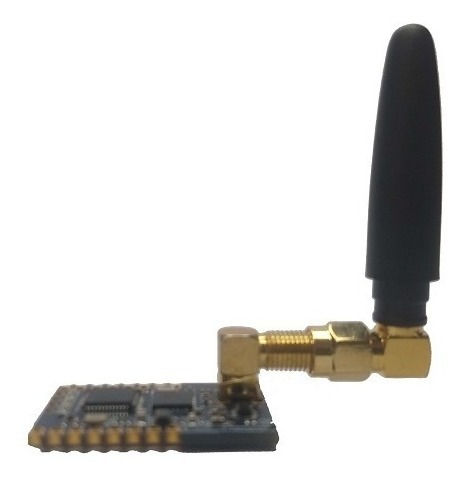
\includegraphics[width=.5\textwidth]{lora}
\end{figure}

\subsubsection{ESP32}\label{ESP32}

\begin{figure}[!h]
  \caption{\label{fig:recivier}ESP32.}
  \centering
  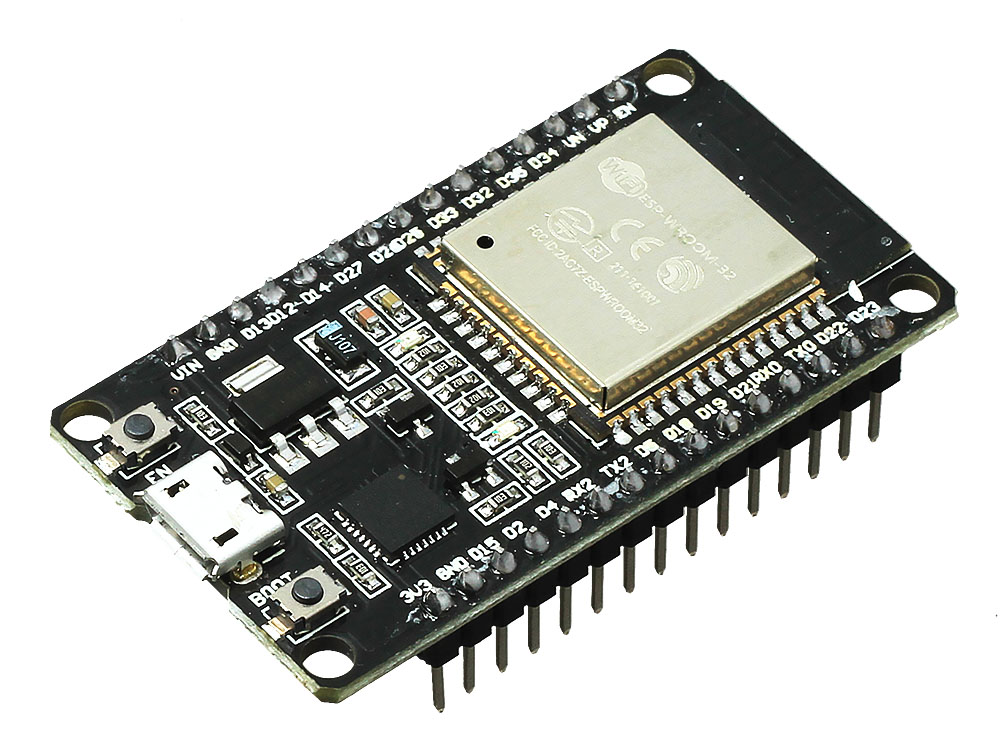
\includegraphics[width=.5\textwidth]{esp}
\end{figure}

\subsubsection{ESP32-CAM}\label{ESP32-CAM}
O dispositivo ESP32-CAM é um controlador embarcado de baixocusto e de baixo consumo energetico

\begin{figure}[!h]
  \caption{\label{fig:recivier}ESP32-CAM.}
  \centering
  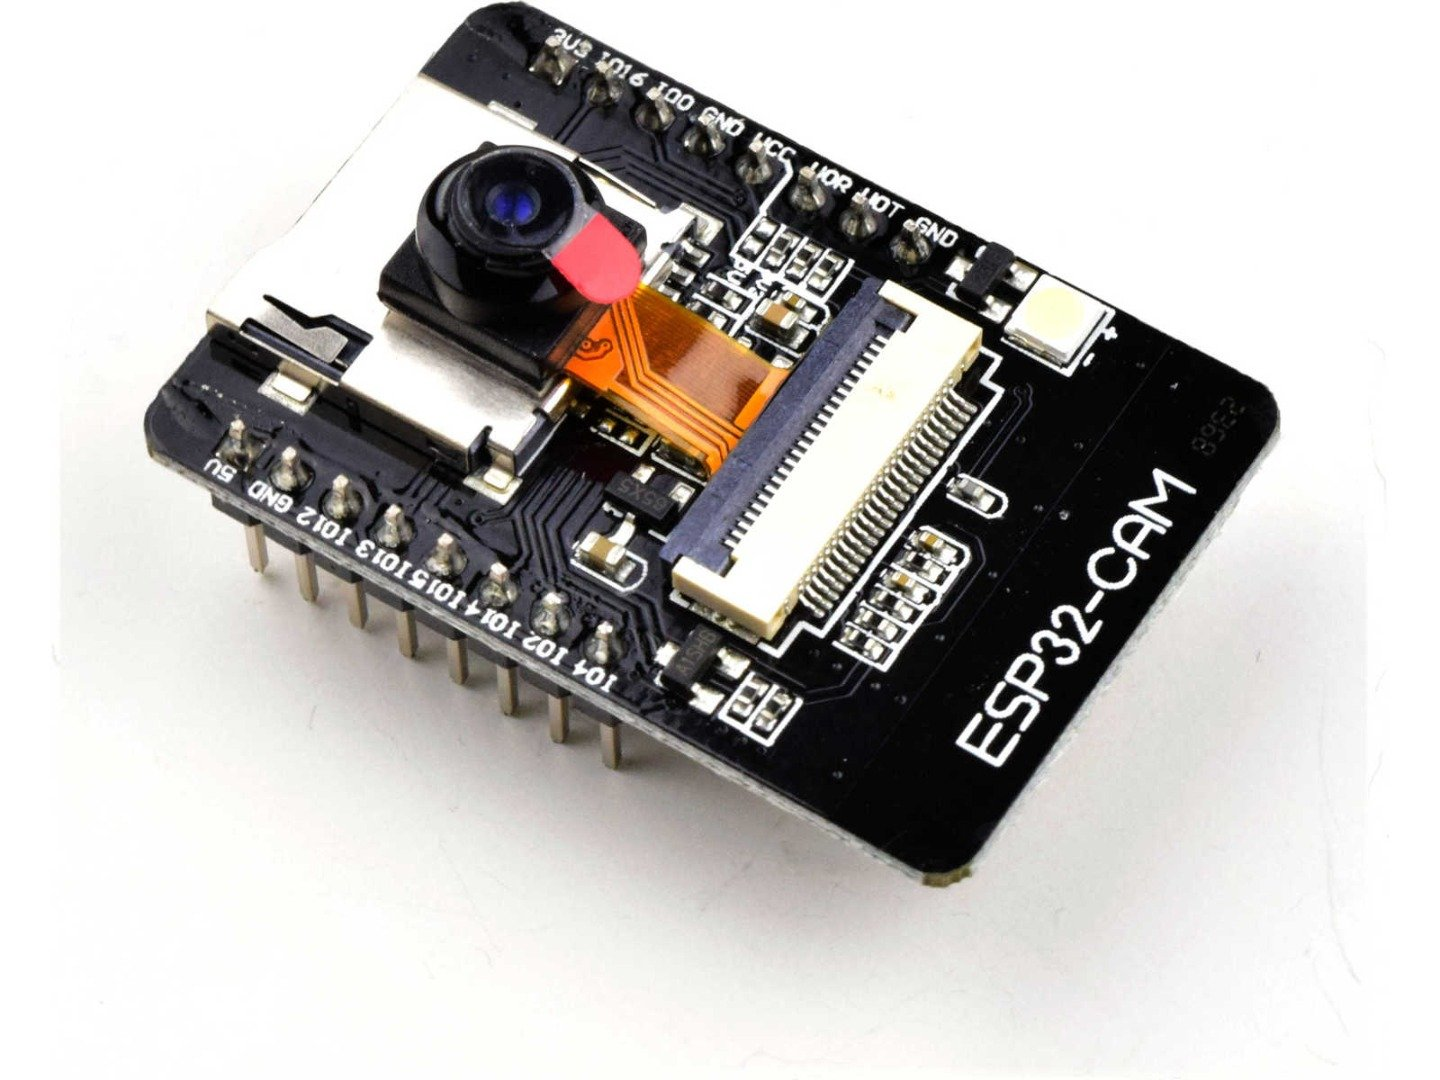
\includegraphics[width=.5\textwidth]{espcam}
\end{figure}

\cleardoublepage

\section{Implementação}

\begin{table}[]
\caption{Estrutura padrão de mensagens LoRa.}
\centering
\begin{tabular}{llll}
\hline
\multicolumn{1}{|c|}{ID}      & \multicolumn{1}{c|}{Command} & \multicolumn{1}{c|}{Payload}       & \multicolumn{1}{c|}{CRC}     \\ \hline
\multicolumn{1}{|c|}{2 bytes} & \multicolumn{1}{c|}{1 byte}  & \multicolumn{1}{c|}{1 - 231 bytes} & \multicolumn{1}{c|}{2 bytes} \\ \hline
 &  &  &  \\
 &  &  &  \\
 &  &  & 
\end{tabular}
\end{table}

\begin{table}[]
\caption{Estrutura definida para o payload da mensagem.}
\centering
\begin{tabular}{cllll}
\hline
\multicolumn{5}{|c|}{Payload}    \\ \hline
\multicolumn{1}{|c|}{Type}   & \multicolumn{1}{c|}{ID}     & \multicolumn{1}{c|}{Part}   & \multicolumn{1}{c|}{Total}  & \multicolumn{1}{c|}{Message}      \\ \hline
\multicolumn{1}{|c|}{1 byte} & \multicolumn{1}{c|}{1 byte} & \multicolumn{1}{c|}{1 byte} & \multicolumn{1}{c|}{1 byte} & \multicolumn{1}{c|}{1 - 227 byte} \\ \hline
\multicolumn{1}{l}{} &  &  &  &  \\
\multicolumn{1}{l}{} &  &  &  & 
\end{tabular}
\end{table}

\begin{lstlisting}[title=Definição da estrutura do payload]
struct _payload {
    uint8_t byte_array[APPLICATION_MAX_PAYLOAD_SIZE];
    uint8_t size;
};

struct _fields {
    uint8_t type;
    uint8_t id;
    uint8_t part;
    uint8_t last_part;
};

union ImagePart {
    _fields fields;
    _payload payload;
};
\end{lstlisting}

\subsection{Sender}

\begin{figure}[!h]
  \caption{\label{fig:sender}Fluxograma geral do algoritmo do sender.}
  \centering
  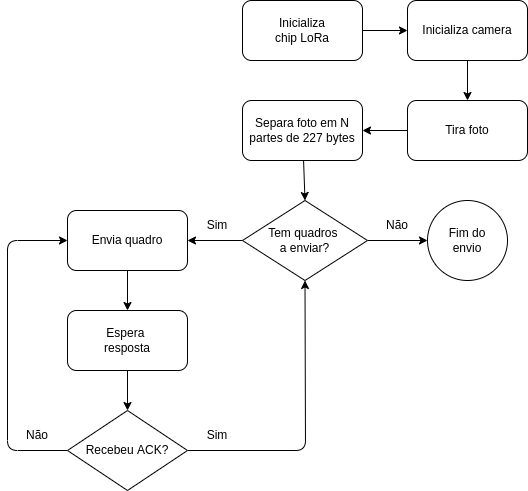
\includegraphics[width=.7\textwidth]{fluxogram_sender}
\end{figure}

\subsection{Reciver}

\begin{figure}[!h]
  \caption{\label{fig:recivier}Fluxograma geral do algoritmo do reciver.}
  \centering
  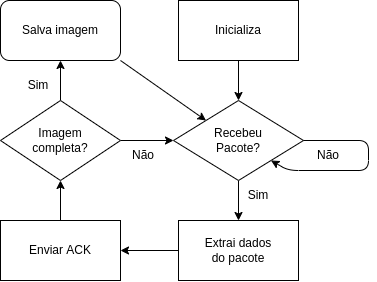
\includegraphics[width=.7\textwidth]{fluxogram_recivier}
\end{figure}

\cleardoublepage

\section{Resultados}

A fim de avaliar o funcionamento da implementação foram realizados diversos testes, dando especial atenção para a forma como a resolução e a taxa de compressão da imagem influenciam no tamanho da mensagem enviada no payload. Os principais resultados são mostrados a continuação.

No primeiro grupo de testes realizado o foco foi avaliar como a resolução da imagem influencia no tamanho em bytes da mensagem enviada. Para isso, 

\begin{table}[]
\centering
\begin{tabular}{@{}c|c@{}}
\toprule
Resolução (pixels) & Tamanho (bytes) \\ \midrule
640x480            & 73260           \\
480x320            & 39139           \\
400x296            & 35916           \\
320x240            & 23510           \\
240x176            & 14242           \\
176x144            & 9147            \\ \bottomrule
\end{tabular}
\caption{Mudança de resolução afetando o tamanho da imagem}
\label{tab:resolution}
\end{table}

\cleardoublepage

\section{Discussão}

% ----------------------------------------------------------
% ELEMENTOS PÓS-TEXTUAIS
% ----------------------------------------------------------

\postextual

% ----------------------------------------------------------
% Referências bibliográficas
% ----------------------------------------------------------
\cleardoublepage
\bibliography{ref}

\end{document}
